%=======================================================================
%  A Unified Projection Framework for Tensor-Structured
%  Dictionary Learning, with an Efficiency Ranking System
%
%  Sahaj Chhetri -- Beamer talk
%  Compiles with pdfLaTeX on Overleaf. All 15 figures live in ./figures/
%=======================================================================
\documentclass[aspectratio=169,9pt]{beamer}

\usetheme{metropolis}
\metroset{
  sectionpage=progressbar,
  subsectionpage=none,
  numbering=fraction,
  progressbar=frametitle,
  block=fill
}

\usepackage[T1]{fontenc}
\usepackage[utf8]{inputenc}
\usepackage{booktabs}
\usepackage{graphicx}
\usepackage{amsmath,amssymb}
\usepackage{tikz}
\usepackage{pgfplots}
\pgfplotsset{compat=1.17}
\usetikzlibrary{arrows.meta,positioning,calc}

%------------------------- palette ------------------------------------
\definecolor{ink}{HTML}{101534}
\definecolor{amber}{HTML}{E8A13A}
\definecolor{teal}{HTML}{2E9E8F}
\definecolor{indigo}{HTML}{2B3A8F}
\definecolor{rust}{HTML}{B34A3F}
\definecolor{lightbg}{HTML}{F3F4F9}
\definecolor{muted}{HTML}{5A6178}

\setbeamercolor{normal text}{fg=ink, bg=white}
\setbeamercolor{alerted text}{fg=amber}
\setbeamercolor{example text}{fg=teal}
\setbeamercolor{frametitle}{bg=ink, fg=white}
\setbeamercolor{progress bar}{fg=amber, bg=ink}
\setbeamercolor{title separator}{fg=amber}
\setbeamercolor{progress bar in head/foot}{fg=amber}
\setbeamercolor{progress bar in section page}{fg=amber}
\setbeamercolor{block title}{bg=lightbg, fg=ink}
\setbeamercolor{block body}{bg=lightbg!55, fg=ink}

% tighter vertical rhythm than the metropolis defaults
\setbeamertemplate{itemize/enumerate body begin}{\small}
\setlength{\parskip}{0.35em}
\addtobeamertemplate{block begin}{\vspace{-0.25em}}{\vspace{-0.15em}}
\addtobeamertemplate{block end}{\vspace{-0.35em}}{}

%------------------------- shorthands ---------------------------------
\newcommand{\dB}{\,dB}
\newcommand{\kr}{\odot}
\newcommand{\kron}{\otimes}
\newcommand{\credit}[1]{{\scriptsize\color{muted}#1}}
\newcommand{\takeaway}[1]{\begin{center}\textit{\small #1}\end{center}}

%------------------------- title --------------------------------------
\title{A Unified Projection Framework for\\Tensor-Structured Dictionary Learning}
\subtitle{Six dictionaries, one harness --- and an efficiency ranking system}
\author{Sahaj Chhetri}
\date{August 17, 2026}

\begin{document}

\maketitle

%=======================================================================
\section{Motivation}
%=======================================================================

\begin{frame}{Flattening a patch discards what made it compressible}
\begin{columns}[T,onlytextwidth]
\begin{column}{0.56\textwidth}
\small
Classical DL models a signal as $y \approx Dx$ with unit-norm atoms and a sparse
code. For a multiway patch the standard recipe flattens it to a vector of length
$n = \prod_i n_i$. Two costs follow:
\begin{itemize}
  \item Spatial neighbourhoods and spectral smoothness --- the redundancy that
        makes the data compressible --- are discarded.
  \item The dictionary carries $n\cdot K$ free numbers, growing
        \emph{multiplicatively} with tensor order.
\end{itemize}
More parameters than the data needs invites over-fitting: the extra capacity is
spent modelling noise.
\end{column}
\begin{column}{0.40\textwidth}
\small
{\color{rust}\Large 25{,}920} \\
\credit{free parameters --- vectorized dictionary, $6\times6\times6$, $K=120$}

\medskip
{\color{teal}\Large 2{,}160} \\
\credit{the same 120 atoms under CP --- $12\times$ smaller}

\medskip
{\color{indigo}\Large 126} \\
\credit{Tucker mode factors covering 343 implicit atoms --- $206\times$}
\end{column}
\end{columns}
\end{frame}

\begin{frame}{Constrain the atom, not the data}
\centering
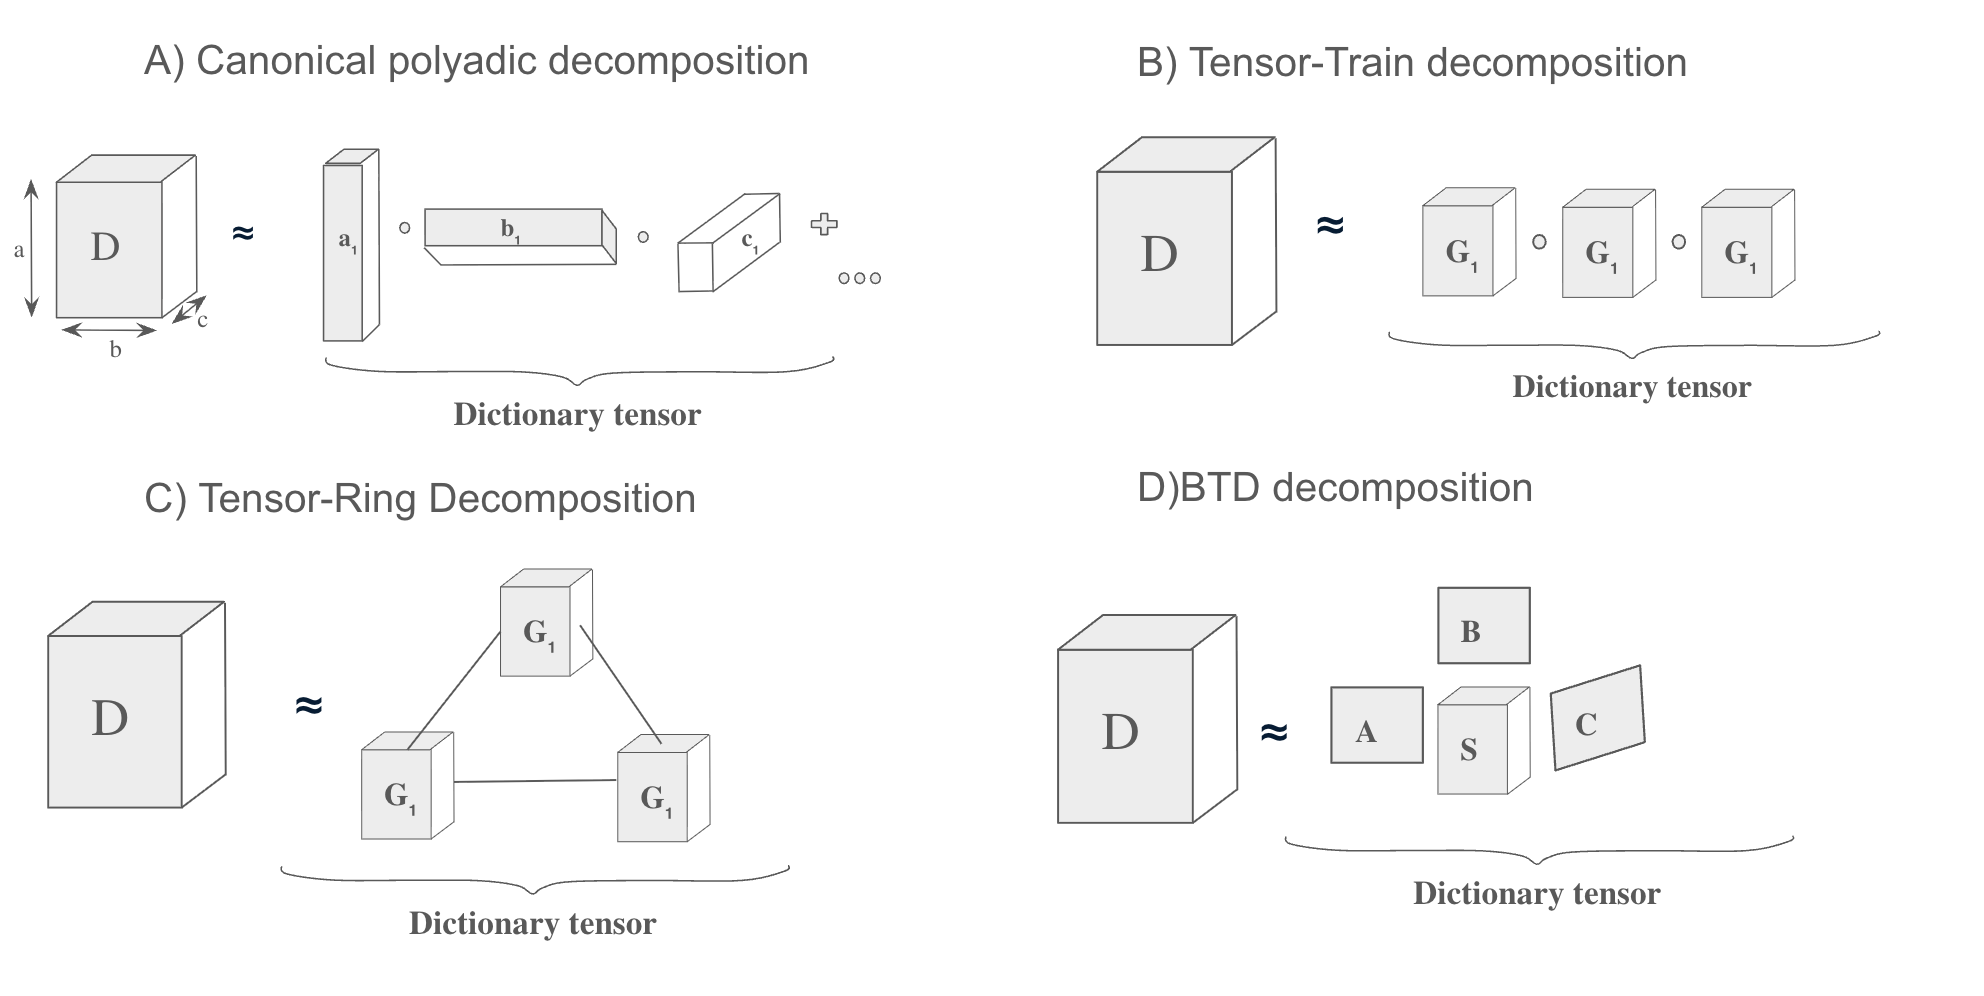
\includegraphics[width=0.74\textwidth]{figures/fig01_decompositions.png}

\credit{Figure 1 --- CP, Tensor-Train, Tensor-Ring and BTD as dictionary tensors.}
\takeaway{Each format represents the same patch at low rank rather than
discarding its structure.}
\end{frame}

\begin{frame}{Contributions}
\begin{columns}[T,onlytextwidth]
\begin{column}{0.48\textwidth}
\begin{block}{1 --- One harness}
\small CP, Tucker, TT, TR, BTD and an unstructured baseline share the same OMP
sparse coding, reconstruction and evaluation.
\end{block}
\begin{block}{2 --- A projection view}
\small CP/TT/TR/BTD are one line changed inside the K-SVD atom update; Tucker is
matched in-harness via separable ALS.
\end{block}
\end{column}
\begin{column}{0.48\textwidth}
\begin{block}{3 --- A ranking system}
\small Three layers, objective to opinionated: Pareto dominance, an
accuracy-per-parameter scalar, profile-weighted tiers.
\end{block}
\begin{block}{4 --- Three regimes}
\small Synthetic mixed-structure patches, real RGB patches and a hyperspectral
cube, plus a matched-budget rate--distortion study.
\end{block}
\end{column}
\end{columns}
\end{frame}

%=======================================================================
\section{The Unified Framework}
%=======================================================================

\begin{frame}{What is held identical, and what is allowed to vary}
\begin{columns}[T,onlytextwidth]
\begin{column}{0.48\textwidth}
\begin{block}{\textcolor{teal}{$=$}\ \ Held identical}
\small
\begin{itemize}
  \item The objective and its solver --- OMP against the effective dictionary $D$
  \item Reconstruction: the map $x \mapsto Dx$
  \item Data, noise level, sparsity cap, seeds
  \item Denoising PSNR against clean held-out patches
\end{itemize}
\end{block}
\end{column}
\begin{column}{0.48\textwidth}
\begin{block}{\textcolor{amber}{$\neq$}\ \ Allowed to vary}
\small
\begin{itemize}
  \item How each atom is parameterized
  \item How many parameters that costs to store
  \item The rank knob each format exposes (CP $R$, TT/TR $r$, BTD $L$)
\end{itemize}
\end{block}
\end{column}
\end{columns}
\takeaway{Each construction usually ships with its own optimizer, so an observed
gap may reflect the optimizer rather than the decomposition. Sharing the solver
makes the comparison apples-to-apples.}
\end{frame}

\begin{frame}{The loop everything plugs into: K-SVD with OMP}
\centering
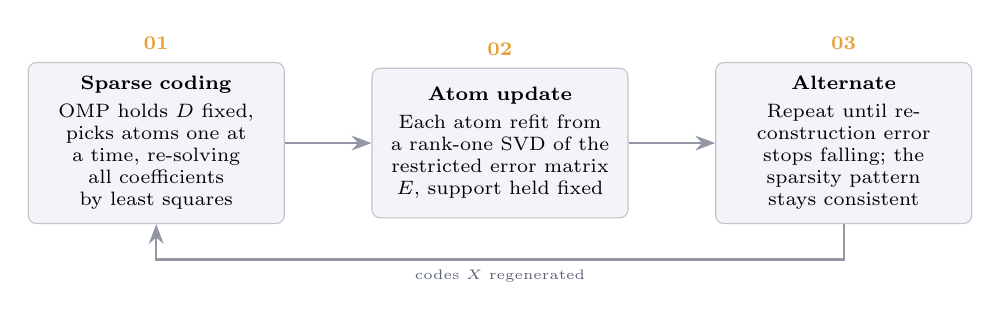
\begin{tikzpicture}[
  node distance=0.8cm and 1.1cm,
  box/.style={rectangle, rounded corners=3pt, draw=ink!25, fill=lightbg,
              text width=2.9cm, minimum height=1.9cm, align=center,
              inner sep=5pt, font=\scriptsize},
  lbl/.style={font=\scriptsize\bfseries, text=amber},
  arr/.style={-{Stealth[length=2.5mm]}, thick, draw=ink!45}
]
\node[box] (a) {\textbf{Sparse coding}\\[2pt]
  OMP holds $D$ fixed, picks atoms one at a time, re-solving all coefficients by
  least squares};
\node[box, right=of a] (b) {\textbf{Atom update}\\[2pt]
  Each atom refit from a rank-one SVD of the restricted error matrix $E$, support
  held fixed};
\node[box, right=of b] (c) {\textbf{Alternate}\\[2pt]
  Repeat until reconstruction error stops falling; the sparsity pattern stays
  consistent};
\node[lbl, above=1pt of a] {01};
\node[lbl, above=1pt of b] {02};
\node[lbl, above=1pt of c] {03};
\draw[arr] (a) -- (b);
\draw[arr] (b) -- (c);
\draw[arr] (c.south) -- ++(0,-0.45) -| node[pos=0.25, below, font=\tiny,
  text=muted] {codes $X$ regenerated} (a.south);
\end{tikzpicture}

\medskip
\begin{block}{The restricted error matrix}
\small
\[ E \;=\; Y_{\Omega} \;-\; D X_{\Omega} \;+\; d_k x_{k,\Omega}^{\top} \]
The final term is easy to misread as \emph{adding} error --- in fact it
un-subtracts atom $k$, leaving the gap a new $d_k$ must fill: the error present
when atom $k$ is \emph{absent}.
\end{block}
\end{frame}

\begin{frame}{Orthogonal matching pursuit, in two mechanics}
\begin{columns}[T,onlytextwidth]
\begin{column}{0.48\textwidth}
\begin{block}{Greedy atom selection}
\small From $r_0 = y$, $\Lambda_0 = \emptyset$, add the best-aligned atom:
\[ \lambda_i = \arg\max_j |\langle d_j, r_{i-1}\rangle|, \quad
   \Lambda_i = \Lambda_{i-1} \cup \{\lambda_i\} \]
\end{block}
\end{column}
\begin{column}{0.48\textwidth}
\begin{block}{Residual update}
\small The whole coefficient vector is recomputed on the active set:
\[ \hat{x} = \arg\min_x \|y - D_{\Lambda_i} x\|_2, \quad
   r_i = y - D_{\Lambda_i}\hat{x} \]
\end{block}
\end{column}
\end{columns}
\takeaway{That orthogonal projection is the defining line: the residual stays
orthogonal to every selected atom, so no atom is chosen twice. The loop stops at
$\|r_i\|_2 < \varepsilon$ or $|\Lambda_i| = s$.}
\end{frame}

\begin{frame}{Where a decomposition can enter}
\begin{columns}[T,onlytextwidth]
\begin{column}{0.48\textwidth}
\begin{block}{On each atom \ \ \textcolor{teal}{\scriptsize CP $\cdot$ TT $\cdot$ TR $\cdot$ BTD}}
\small Each atom is itself a low-parameter tensor. Atoms are independent, so the
constraint is enforced atom-by-atom: \emph{snap} the optimal unconstrained atom
onto the decomposition's manifold.
\[ D = A \kr B \kr C \quad \text{\scriptsize (Khatri--Rao)} \]
\credit{Storage falls from $n_1 n_2 n_3 K$ to $(n_1{+}n_2{+}n_3)K$.}
\end{block}
\end{column}
\begin{column}{0.48\textwidth}
\begin{block}{On the whole dictionary \ \ \textcolor{amber}{\scriptsize TUCKER}}
\small Every atom is built from one shared set of per-mode vectors, so the
constraint couples all atoms. The update re-fits the shared mode factors by
separable ALS.
\[ D = U_3 \kron U_2 \kron U_1 \quad \text{\scriptsize (Kronecker)} \]
\credit{The core plays the role of the sparse code.}
\end{block}
\end{column}
\end{columns}
\takeaway{The Khatri--Rao is the column-matched Kronecker: CP keeps only matched
triples, Tucker keeps all $k_1 k_2 k_3$ combinations.}
\end{frame}

\begin{frame}{Tucker in the same harness}
\begin{columns}[T,onlytextwidth]
\begin{column}{0.52\textwidth}
\small
Same outer loop --- OMP against $D = U_3 \kron U_2 \kron U_1$, giving each sample
a sparse core --- then update the mode factors by separable ALS. Holding the
cores fixed, each $U_n$ minimizes
\[ \sum_m \big\| \mathcal{Y}_m - \mathcal{C}_m \times_1 U_1 \times_2 U_2 \times_3 U_3 \big\|^2 , \]
which for mode $n$ is the linear solve
\[ U_n = X_n G_n^{\top}\big(G_n G_n^{\top} + \lambda I\big)^{-1},
   \quad G_m = \mathcal{C}_m \times_{p \neq n} U_p . \]
\credit{This ``re-fit the shared factors'' step is the Tucker analogue of the
per-atom snap, and the canonical separable/Kronecker construction.}
\end{column}
\begin{column}{0.44\textwidth}
\centering
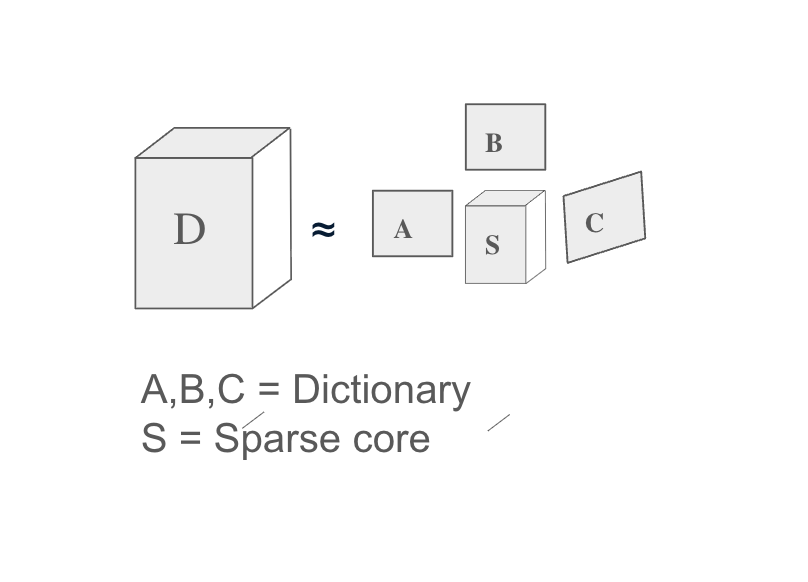
\includegraphics[width=0.86\textwidth]{figures/fig02_tucker_dictionary.png}

\credit{Figure 2 --- the core is the sparse matrix; the three mode matrices are
the dictionary.}
\end{column}
\end{columns}
\end{frame}

\begin{frame}{Parameter accounting}
\centering
\small
\begin{tabular}{@{}lll@{}}
\toprule
\textbf{Method} & \textbf{Dictionary form} & \textbf{Stored parameters} \\
\midrule
Vectorized             & free atoms                                     & $K \prod_i n_i$ \\
CP (rank $R$)          & $D = A \kr B \kr C$ \ (Khatri--Rao)            & $K R S$ \\
Tucker                 & $D = U_N \kron \cdots \kron U_1$ \ (Kronecker) & $\sum_i n_i k_i$ \\
TT (rank $r$, $N{=}3$) & chain of cores                                 & $K\big[r(n_1{+}n_3) + r^2 n_2\big]$ \\
TR (rank $r$)          & ring of cores                                  & $K r^2 S$ \\
BTD ($L$, $b$ blocks)  & sum of Tucker blocks                           & $K b (L^N + L S)$ \\
\bottomrule
\end{tabular}

\medskip
\credit{Table 1 --- $S = \sum_i n_i$, atom shape $(n_1,\dots,n_N)$. The sparse
code (or Tucker core) is per-sample and excluded from every method equally. For
Tucker the atom count is $\prod_i k_i$; only the mode factors are stored.}
\takeaway{Every count is multiplicative in $K$ except Tucker's, which is additive
across modes --- that single asymmetry drives much of what follows.}
\end{frame}

%=======================================================================
\section{Efficiency Ranking System}
%=======================================================================

\begin{frame}{Layer 1: Pareto dominance (weight-free)}
\begin{columns}[T,onlytextwidth]
\begin{column}{0.42\textwidth}
\small
On the two core axes --- test accuracy and parameter-efficiency --- a method is
\emph{dominated} if another is at least as good on both and strictly better on
one.
\medskip

No non-negative weighting can rescue a dominated method, so this layer holds
regardless of anyone's priorities.
\medskip

The non-dominated methods form the rate--distortion frontier; Layers 2 and 3 only
rank what survives here.
\end{column}
\begin{column}{0.56\textwidth}
\centering
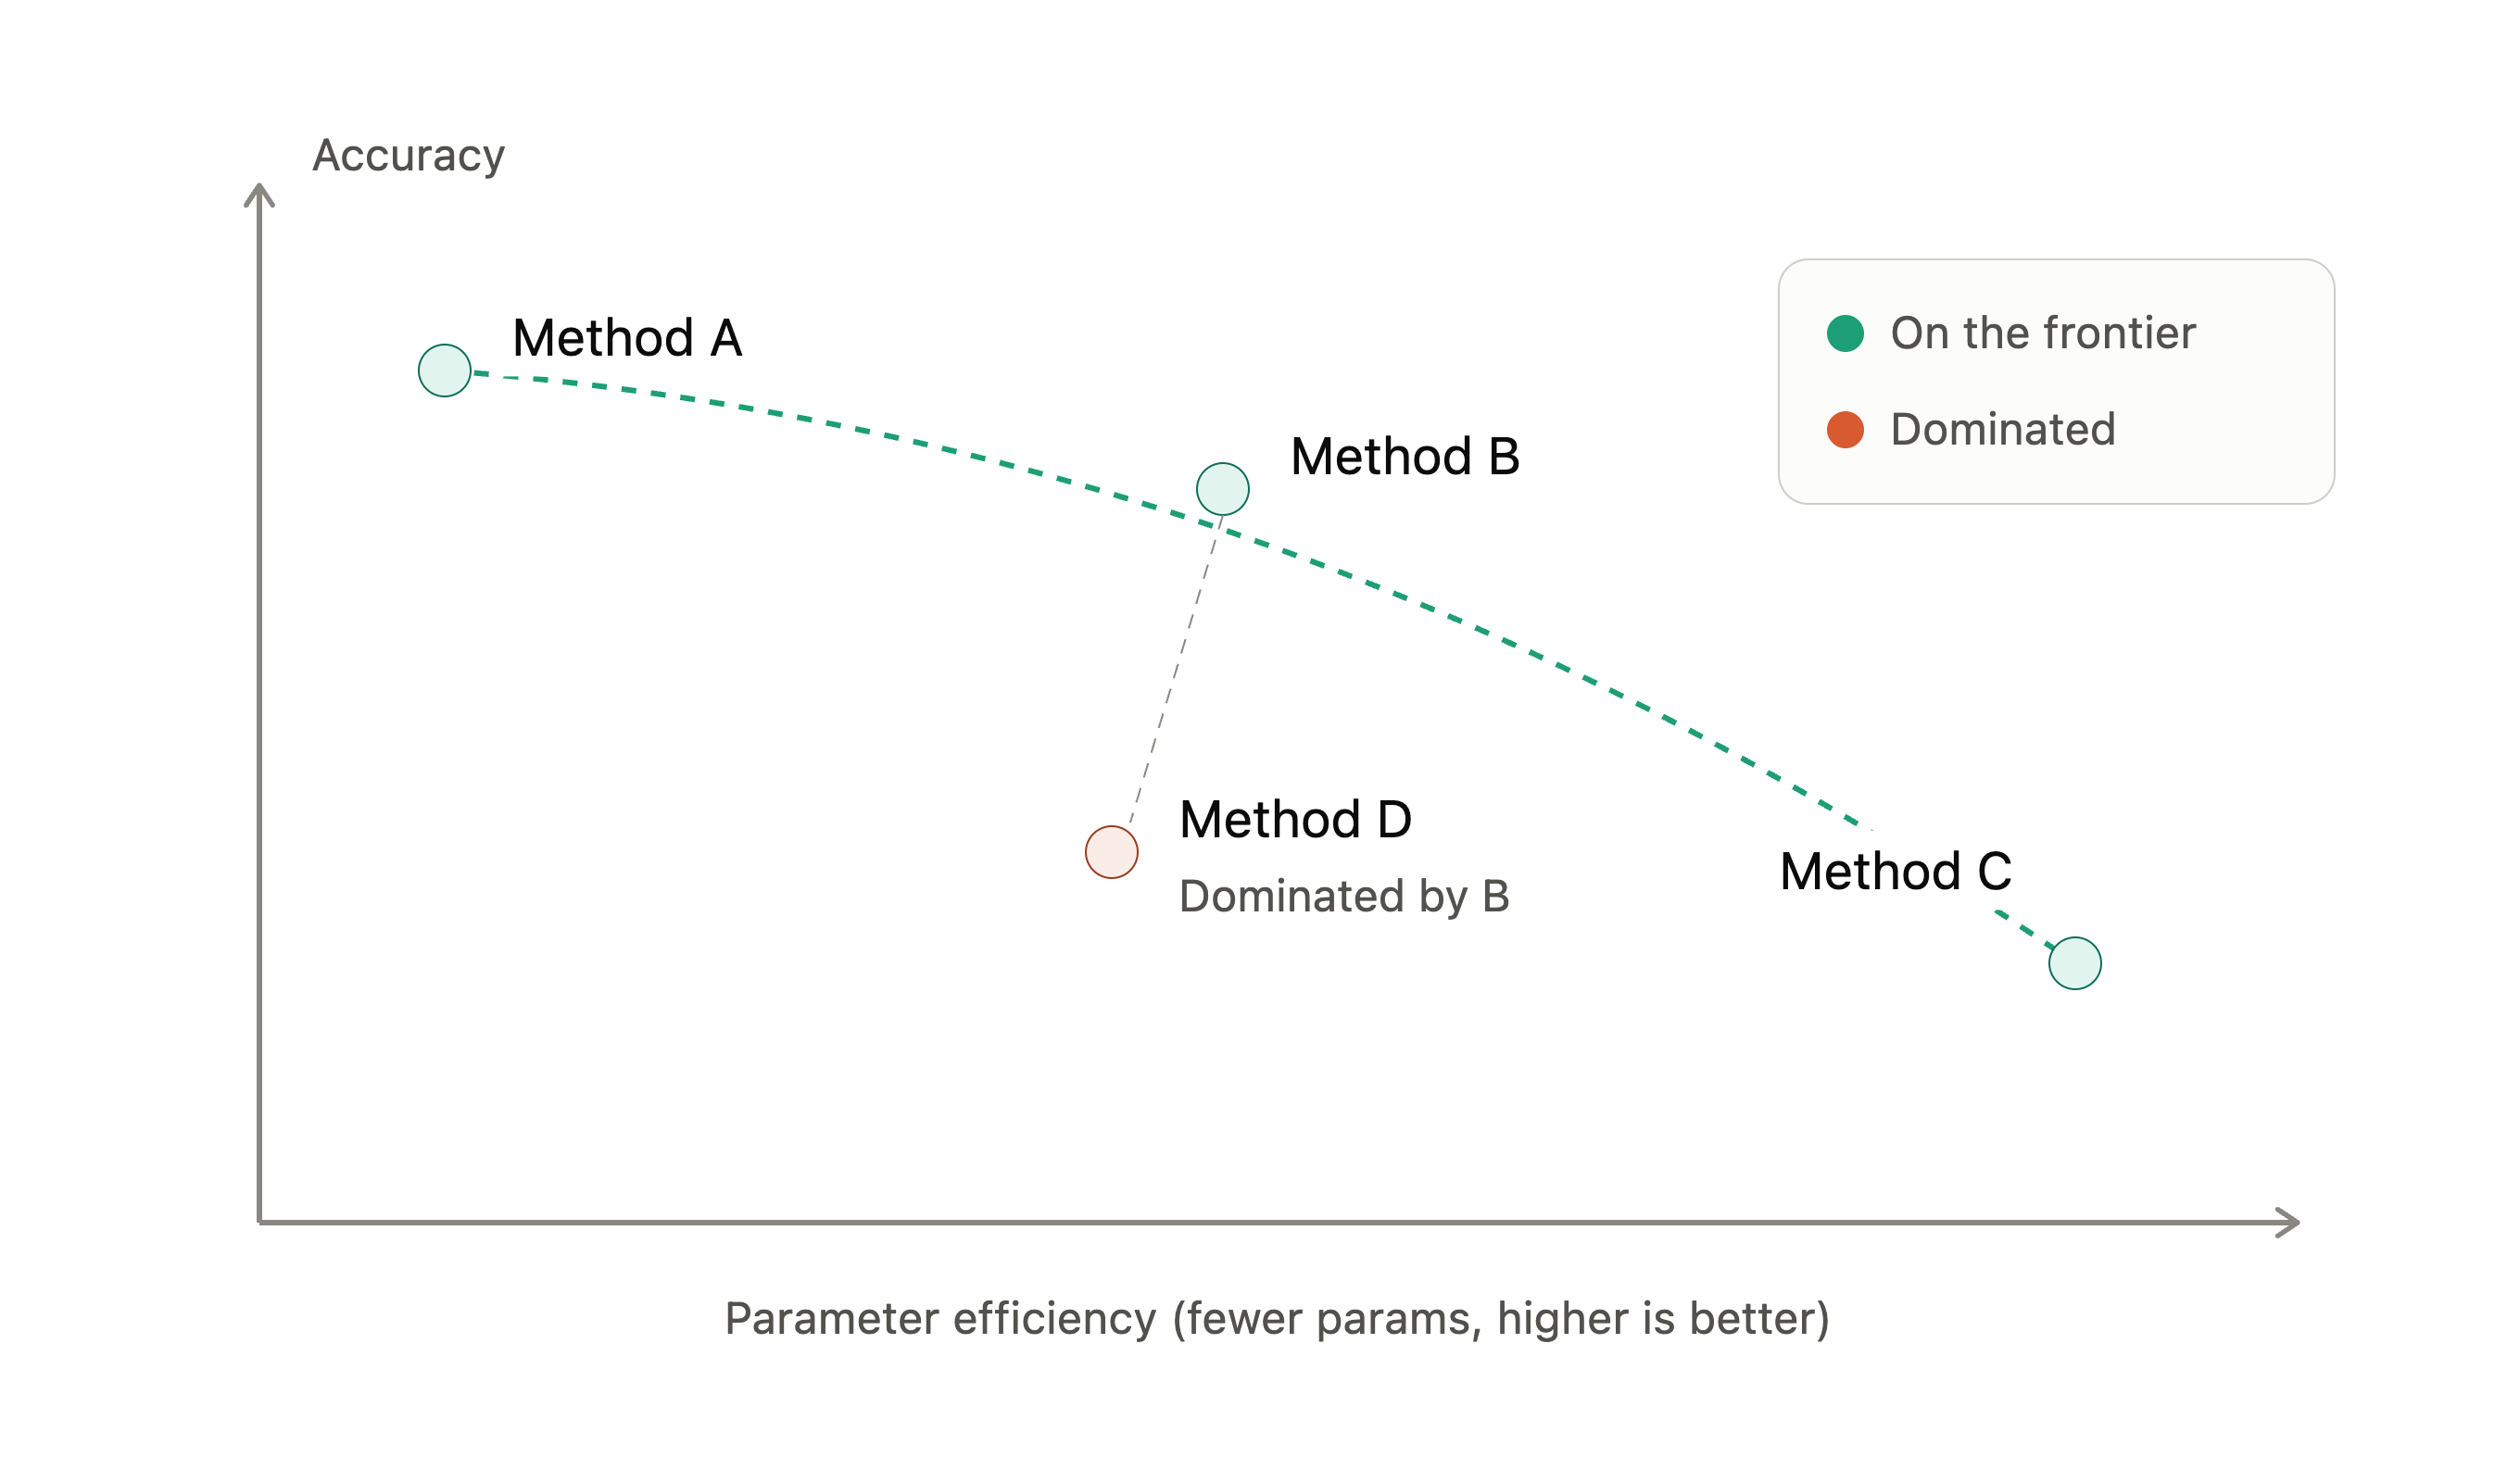
\includegraphics[width=0.94\textwidth]{figures/fig03_pareto_concept.png}

\credit{Figure 3 --- Method D is dominated by B; A, B and C form the frontier.}
\end{column}
\end{columns}
\end{frame}

\begin{frame}{Layers 2 and 3: a scalar, then a profile}
\begin{columns}[T,onlytextwidth]
\begin{column}{0.44\textwidth}
\begin{block}{Layer 2 --- an interpretable scalar}
\small
\[ \mathbf{E} \;=\; \frac{\mathrm{PSNR}}{\log_{10}(\mathrm{params})} \]
with $\mathrm{MSE} = \tfrac{1}{N}\sum_i (x_i - \hat{x}_i)^2$ and
$\mathrm{PSNR} = 10\log_{10}(\mathrm{MAX}^2/\mathrm{MSE})$.
The denominator counts \emph{decades} of parameters, so $E$ reads as decibels of
fidelity per order of magnitude spent.
\end{block}
\end{column}
\begin{column}{0.52\textwidth}
\begin{block}{Layer 3 --- profile-weighted tiers}
\centering\scriptsize
\begin{tabular}{@{}lcccc@{}}
\toprule
\textbf{Profile} & \textbf{Acc.} & \textbf{Par.} & \textbf{Speed} & \textbf{Rob.}\\
\midrule
Balanced           & 0.40 & 0.30 & 0.15 & 0.15 \\
Quality (offline)  & 0.60 & 0.20 & 0.10 & 0.10 \\
Compression (edge) & 0.25 & 0.55 & 0.10 & 0.10 \\
Realtime           & 0.30 & 0.20 & 0.40 & 0.10 \\
\bottomrule
\end{tabular}

\smallskip
Each axis min--max normalized to $[0,1]$, then graded $S \geq 0.80$,
$A \geq 0.65$, $B \geq 0.45$, $C \geq 0.25$, else $D$.
\end{block}
\end{column}
\end{columns}
\end{frame}

%=======================================================================
\section{Experimental Setup}
%=======================================================================

\begin{frame}{Three datasets, three different questions}
\small
\begin{block}{Synthetic mixed-structure --- $6\times6\times6$}
\small 40\% separable (rank-one), 40\% low-TT-rank, 20\% dense, so no structure
is trivially favoured. We sweep the rank directly rather than tiering one
hand-picked configuration.
\end{block}
\begin{block}{Real RGB patches --- $8\times8\times3$}
\small From a standard photograph, mean-removed and normalized. No ground truth,
so the full three-layer ranking is applied at fixed hyperparameters.
\end{block}
\begin{block}{Hyperspectral cube --- $6\times6\times16$}
\small Genuinely low-rank with one fat spectral mode. Evaluated at matched
parameter budget, so we report the frontier rather than tier scores.
\end{block}
\credit{Dictionaries are learned on noisy training patches and evaluated by
denoising PSNR against clean held-out test patches, averaged over seeds.
Decomposition primitives use TensorLy.}
\end{frame}

\begin{frame}{The synthetic hyperspectral cube}
\centering
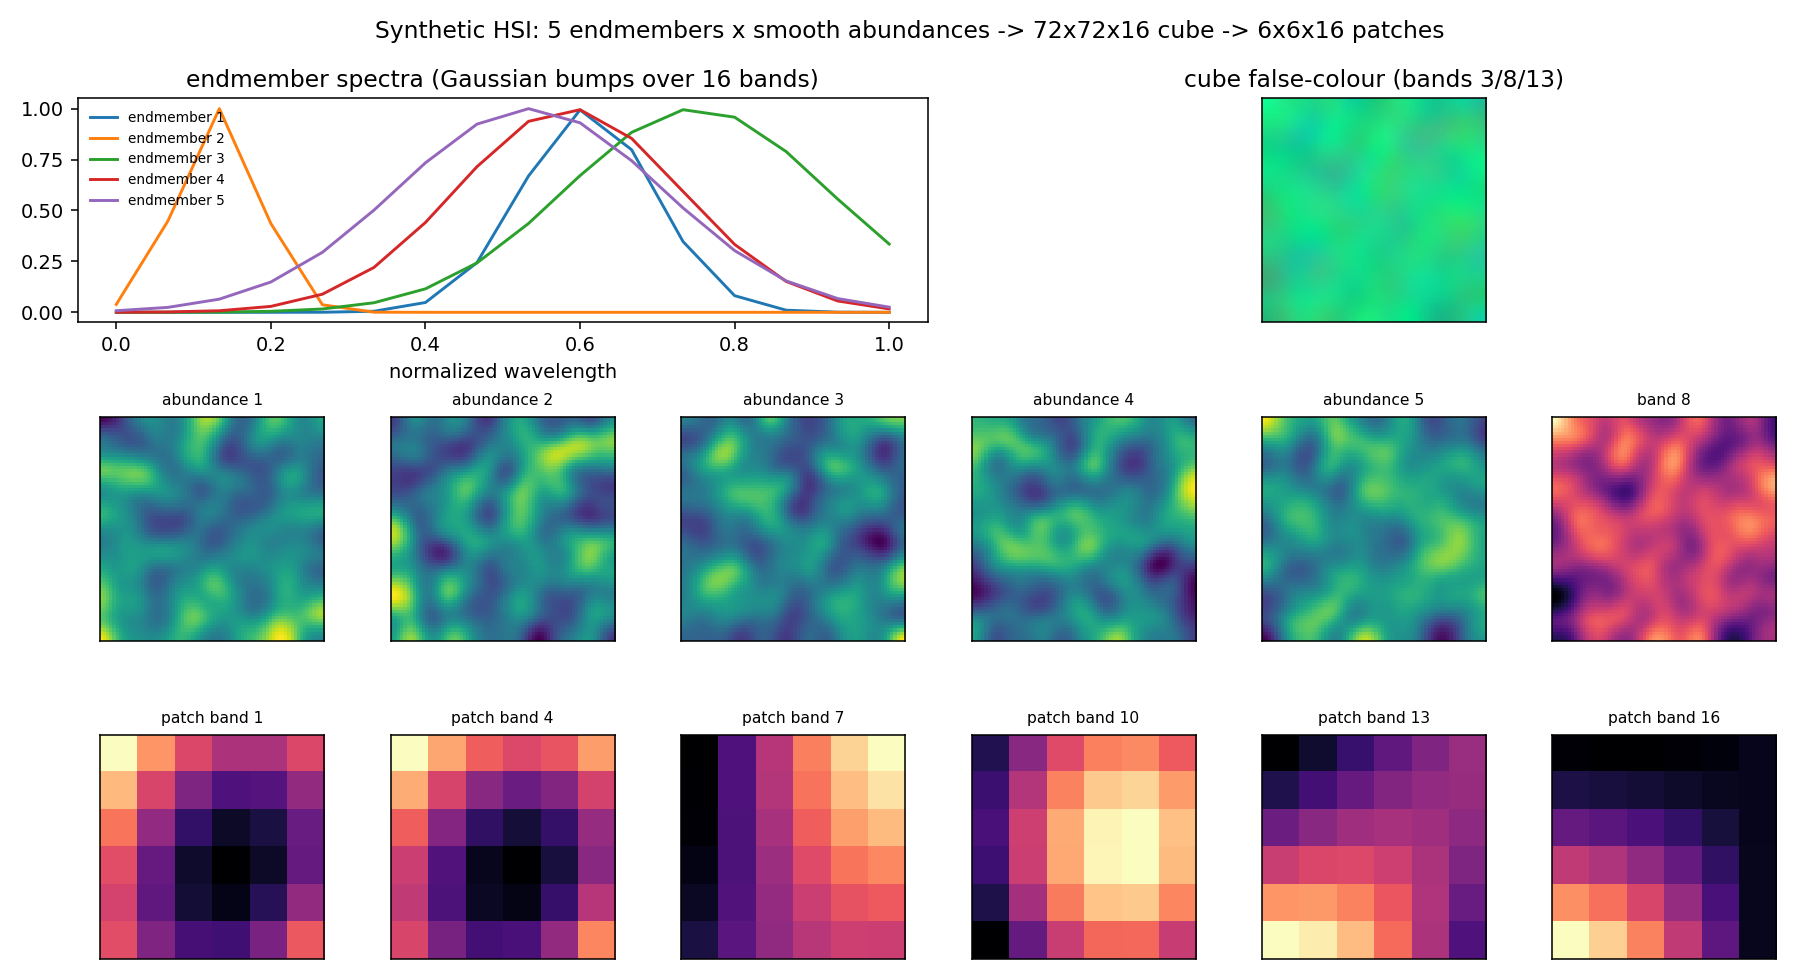
\includegraphics[width=0.60\textwidth]{figures/fig15_hsi_cube.png}

\credit{Figure 15 --- five Gaussian endmember spectra mixed by smooth abundance
maps into a $72\times72\times16$ cube (false-colour composite shown), cut into
$6\times6\times16$ patches. Genuinely low-rank with one fat spectral mode; no
real HSI capture is used.}
\end{frame}

\begin{frame}{The real RGB patches}
\centering
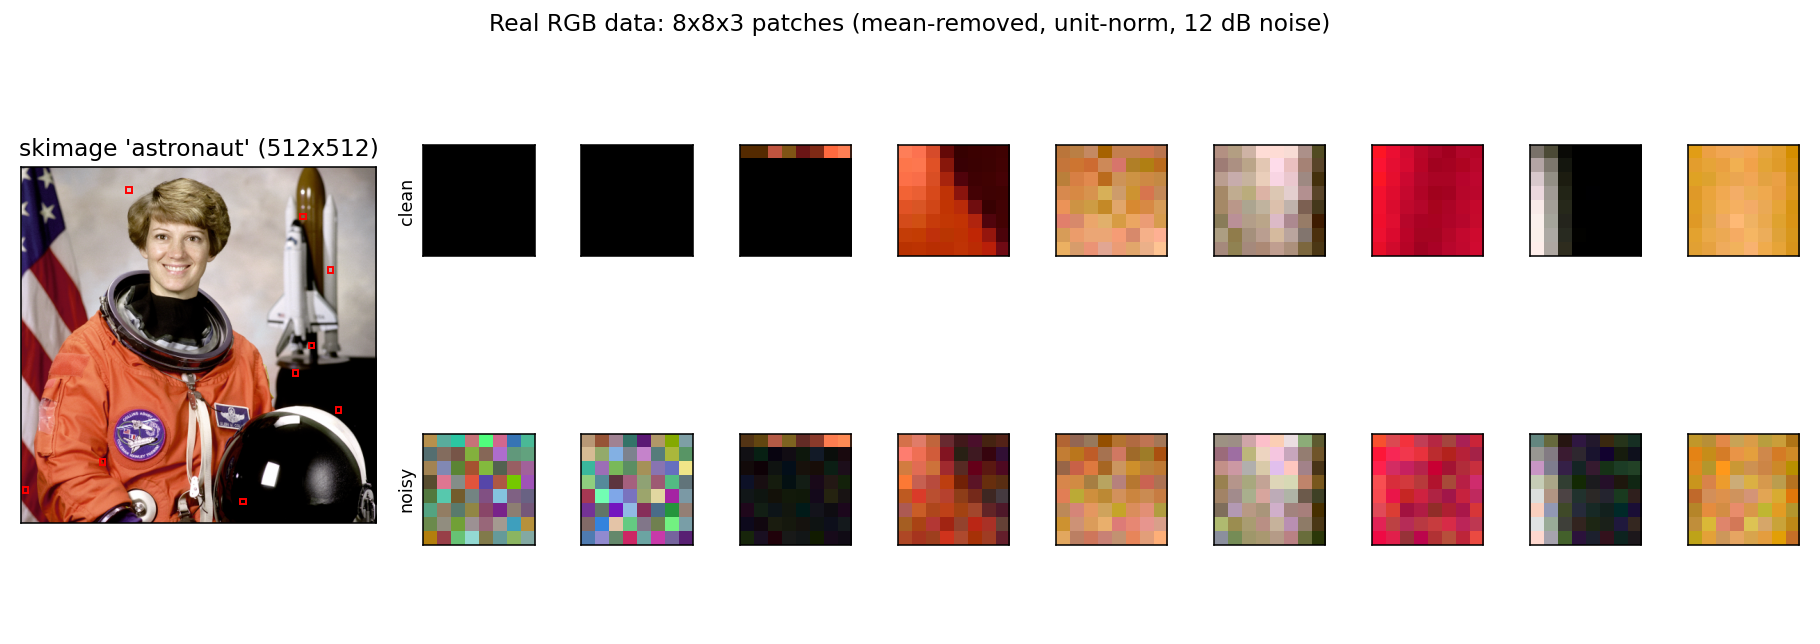
\includegraphics[width=0.90\textwidth]{figures/fig08_rgb_data.png}

\credit{Figure 8 --- the skimage astronaut image with sampled $8\times8\times3$
patch locations, and clean/noisy patch pairs.}
\takeaway{Natural patches are smooth and approximately low-rank --- the regime
where structural constraints regularize rather than restrict.}
\end{frame}

%=======================================================================
\section{Results 1: Synthetic Data}
%=======================================================================

\begin{frame}{On rich, clean data the unstructured baseline wins}
\begin{columns}[T,onlytextwidth]
\begin{column}{0.50\textwidth}
\centering\small
\begin{tabular}{@{}lrrrr@{}}
\toprule
\textbf{Model} & \textbf{Atoms} & \textbf{Params} & \textbf{Fit (s)} & \textbf{PSNR} \\
\midrule
Vectorized      & 120 & 25{,}920 & 0.85 & \textbf{41.49} \\
CP              & 120 &  2{,}160 & 3.50 & 33.14 \\
Tucker$^\dagger$& 343 &      126 & 1.42 & 27.01 \\
TT              & 120 &  5{,}760 & 1.13 & 38.29 \\
TR              & 120 &  8{,}640 & 1.24 & 38.95 \\
\bottomrule
\end{tabular}

\medskip
\credit{Table 3 --- $6\times6\times6$, 12\dB, $K{=}120$, sparsity 6, 5 seeds.
$^\dagger$initial out-of-harness optimizer; corrected later.}
\end{column}
\begin{column}{0.46\textwidth}
\centering
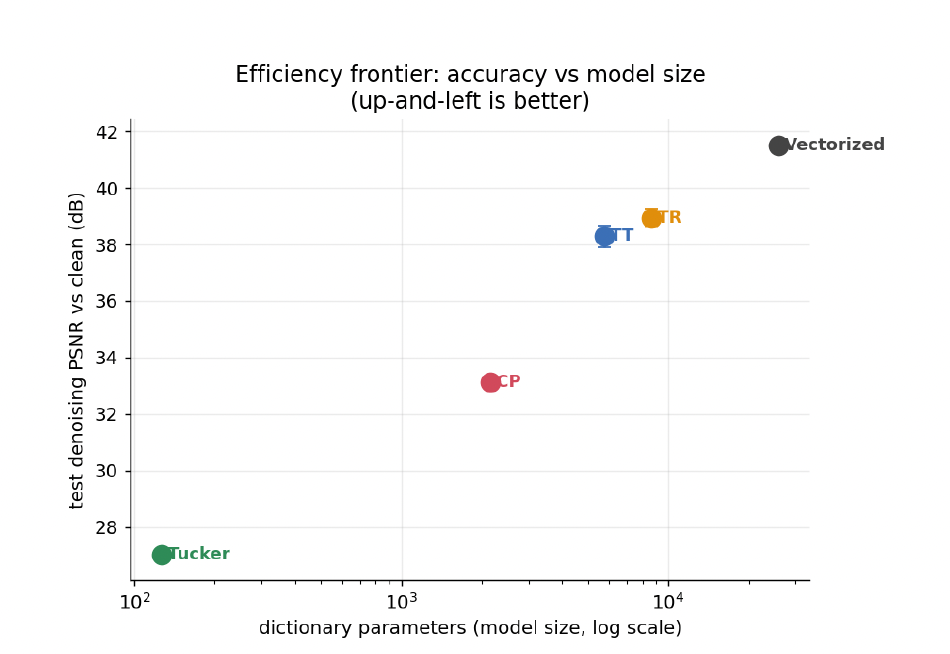
\includegraphics[width=0.86\textwidth]{figures/fig05_frontier_synthetic.png}

\credit{Figure 5 --- up-and-left is better.}
\end{column}
\end{columns}
\takeaway{The baseline buys 41.5\dB{} with the largest dictionary by an order of
magnitude; CP is most compact per atom but least accurate at fixed atom count.}
\end{frame}

\begin{frame}{Because 20\% of the signal has no tensor structure to exploit}
\centering
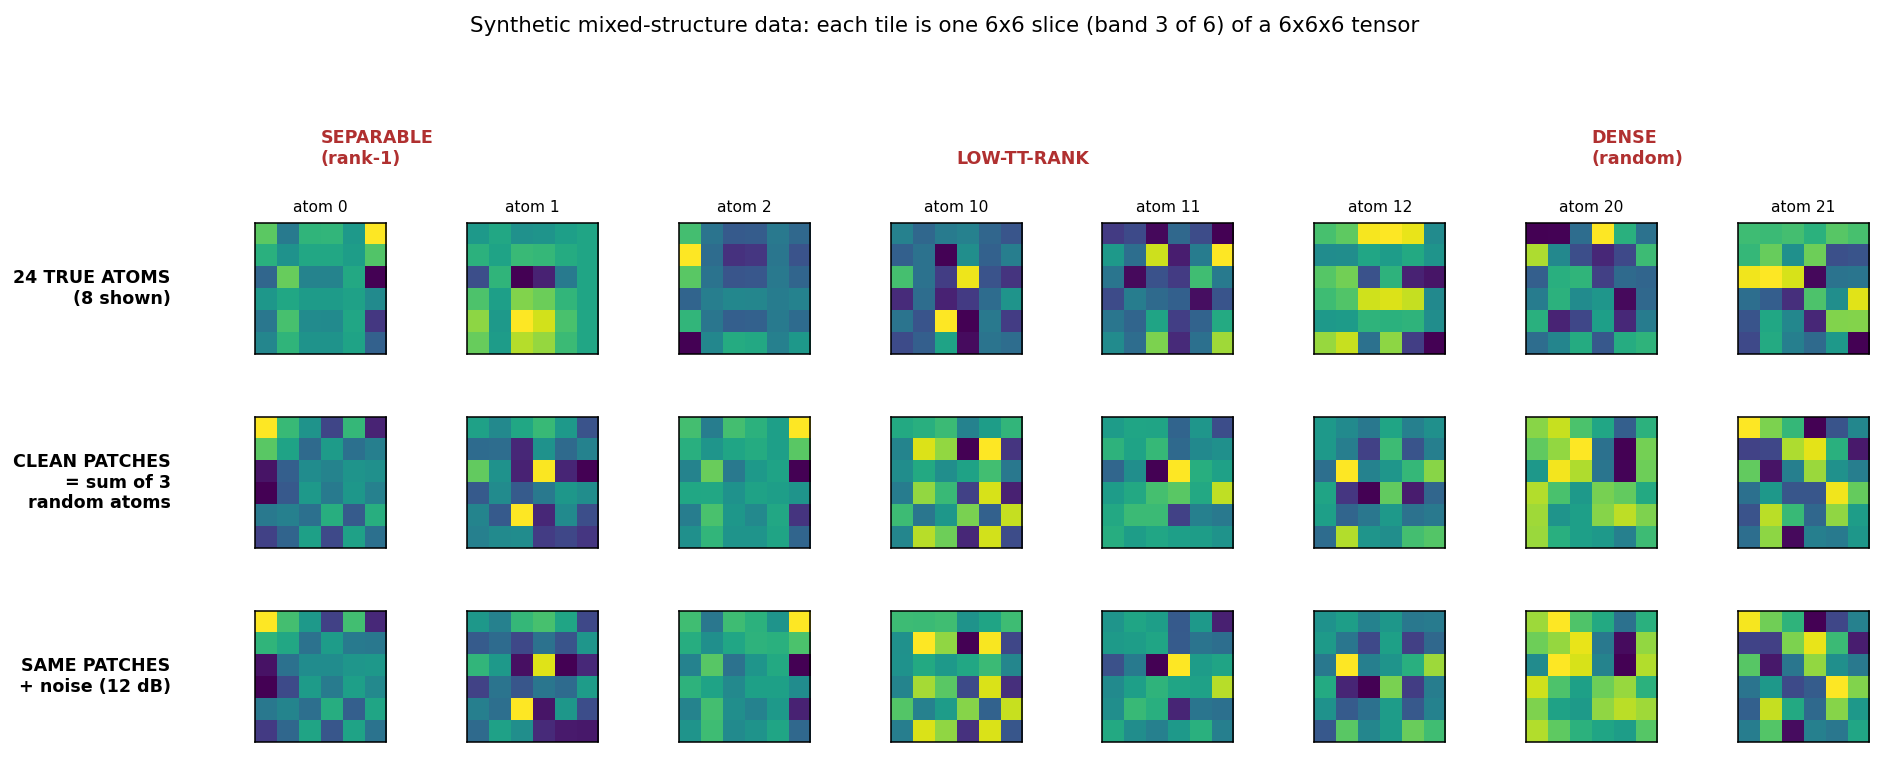
\includegraphics[width=0.82\textwidth]{figures/fig04_synthetic_atoms.png}

\credit{Figure 4 --- eight of the 24 ground-truth atoms (separable /
low-TT-rank / dense), clean patches formed as sums of three atoms, and their
12\dB{} noisy versions.}
\takeaway{Any method constraining atoms to a tensor format is limited on the
dense fifth of the data. At 12\dB{} noise imposes no strong regularization, so
the baseline's extra freedom converts directly into accuracy.}
\end{frame}

\begin{frame}{Rank sensitivity: where the formats separate}
\centering
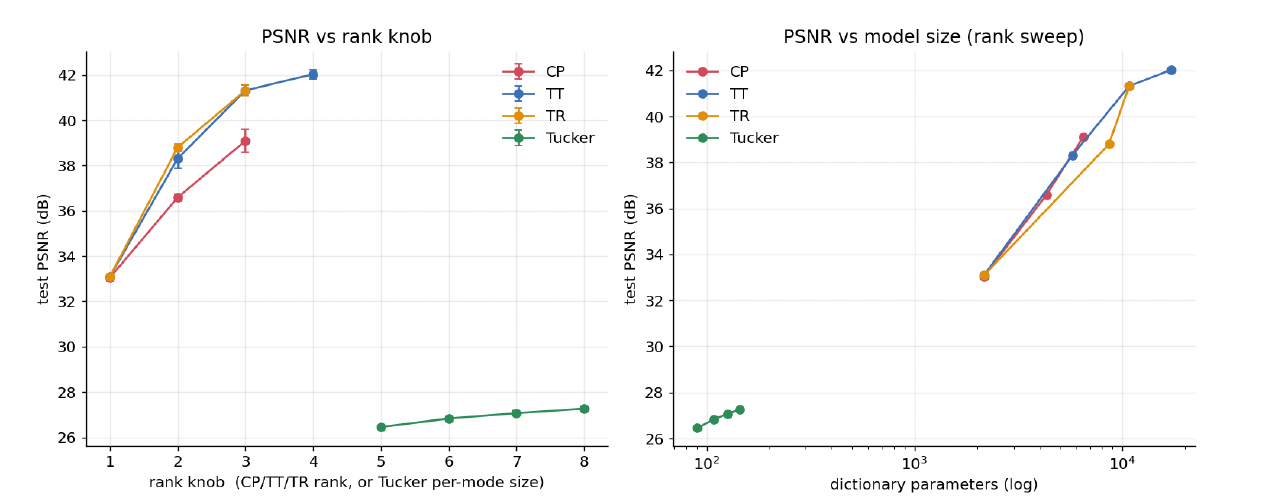
\includegraphics[width=0.86\textwidth]{figures/fig06_rank_sensitivity.png}

\credit{Figure 6 --- left: PSNR versus each method's rank knob. Right: PSNR
versus dictionary parameters under the rank sweep.}

\smallskip
\scriptsize
CP, TT and TR start at the identical point ($\approx 33.1\dB$) at rank 1 --- there
the three decompositions coincide, each expanding into the same outer product
$a \circ b \circ c$. CP then lags, sitting $\approx 2\dB$ below TT/TR at rank 2
(36.6 vs 38.3--38.8) and needing rank 3 to reach 39\dB. TT overtakes the baseline
at rank 4.
\end{frame}

\begin{frame}{Constraint buys stability across initializations}
\begin{columns}[T,onlytextwidth]
\begin{column}{0.50\textwidth}
\centering
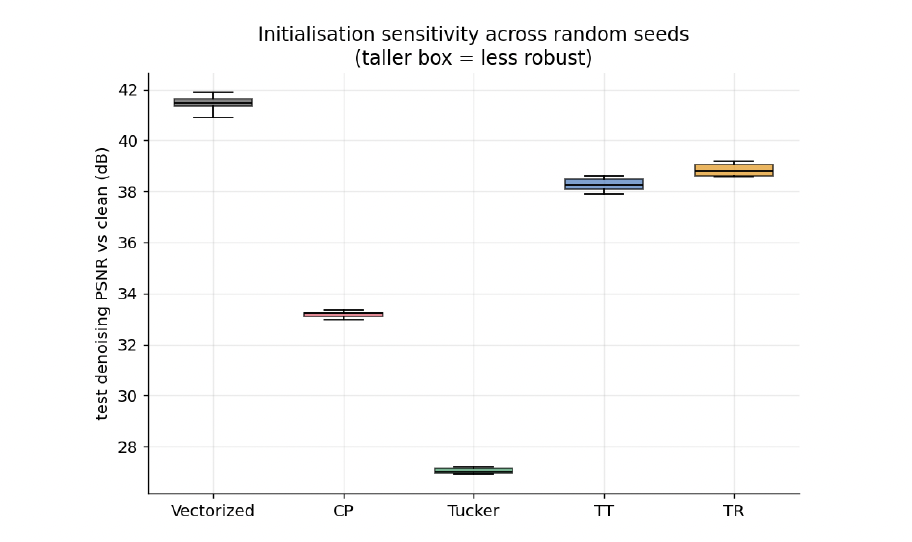
\includegraphics[width=0.90\textwidth]{figures/fig07_init_sensitivity.png}

\credit{Figure 7 --- taller box = more sensitive to the random seed.}
\end{column}
\begin{column}{0.46\textwidth}
\small
\begin{itemize}
  \item Each method is run over multiple seeds; the spread of resulting PSNR is
        plotted as a box.
  \item The baseline varies most; constrained models converge to roughly the same
        answer regardless of initialization.
  \item CP's wide bars are the fingerprint of ALS without an SVD warm start; TT
        and TR fit by truncation.
\end{itemize}
\medskip
\begin{alertblock}{}
\small Seed variance is often a readout of \emph{optimiser} quality, not
\emph{model} quality.
\end{alertblock}
\end{column}
\end{columns}
\end{frame}

%=======================================================================
\section{Results 2: Real RGB Patches}
%=======================================================================

\begin{frame}{On real patches the conclusion inverts}
\begin{columns}[T,onlytextwidth]
\begin{column}{0.50\textwidth}
\centering\small
\begin{tabular}{@{}lrrrr@{}}
\toprule
\textbf{Model} & \textbf{Params} & \textbf{Compr.} & \textbf{Fit (s)} & \textbf{PSNR} \\
\midrule
Vectorized       & 19{,}200 & $1.0\times$   & 0.82 & 30.81 \\
CP               &  1{,}900 & $10.1\times$  & 2.54 & \textbf{31.65} \\
Tucker$^\dagger$ &      153 & $125.5\times$ & 1.41 & 30.74 \\
TT               &  5{,}400 & $3.6\times$   & 1.06 & 31.27 \\
TR               &  7{,}600 & $2.5\times$   & 1.18 & 31.27 \\
BTD              &  4{,}600 & $4.2\times$   & 3.00 & 31.37 \\
\bottomrule
\end{tabular}

\medskip
\credit{Table 4 --- $8\times8\times3$, 12\dB, sparsity 6.
$^\dagger$initial out-of-harness optimizer.}
\end{column}
\begin{column}{0.46\textwidth}
\centering
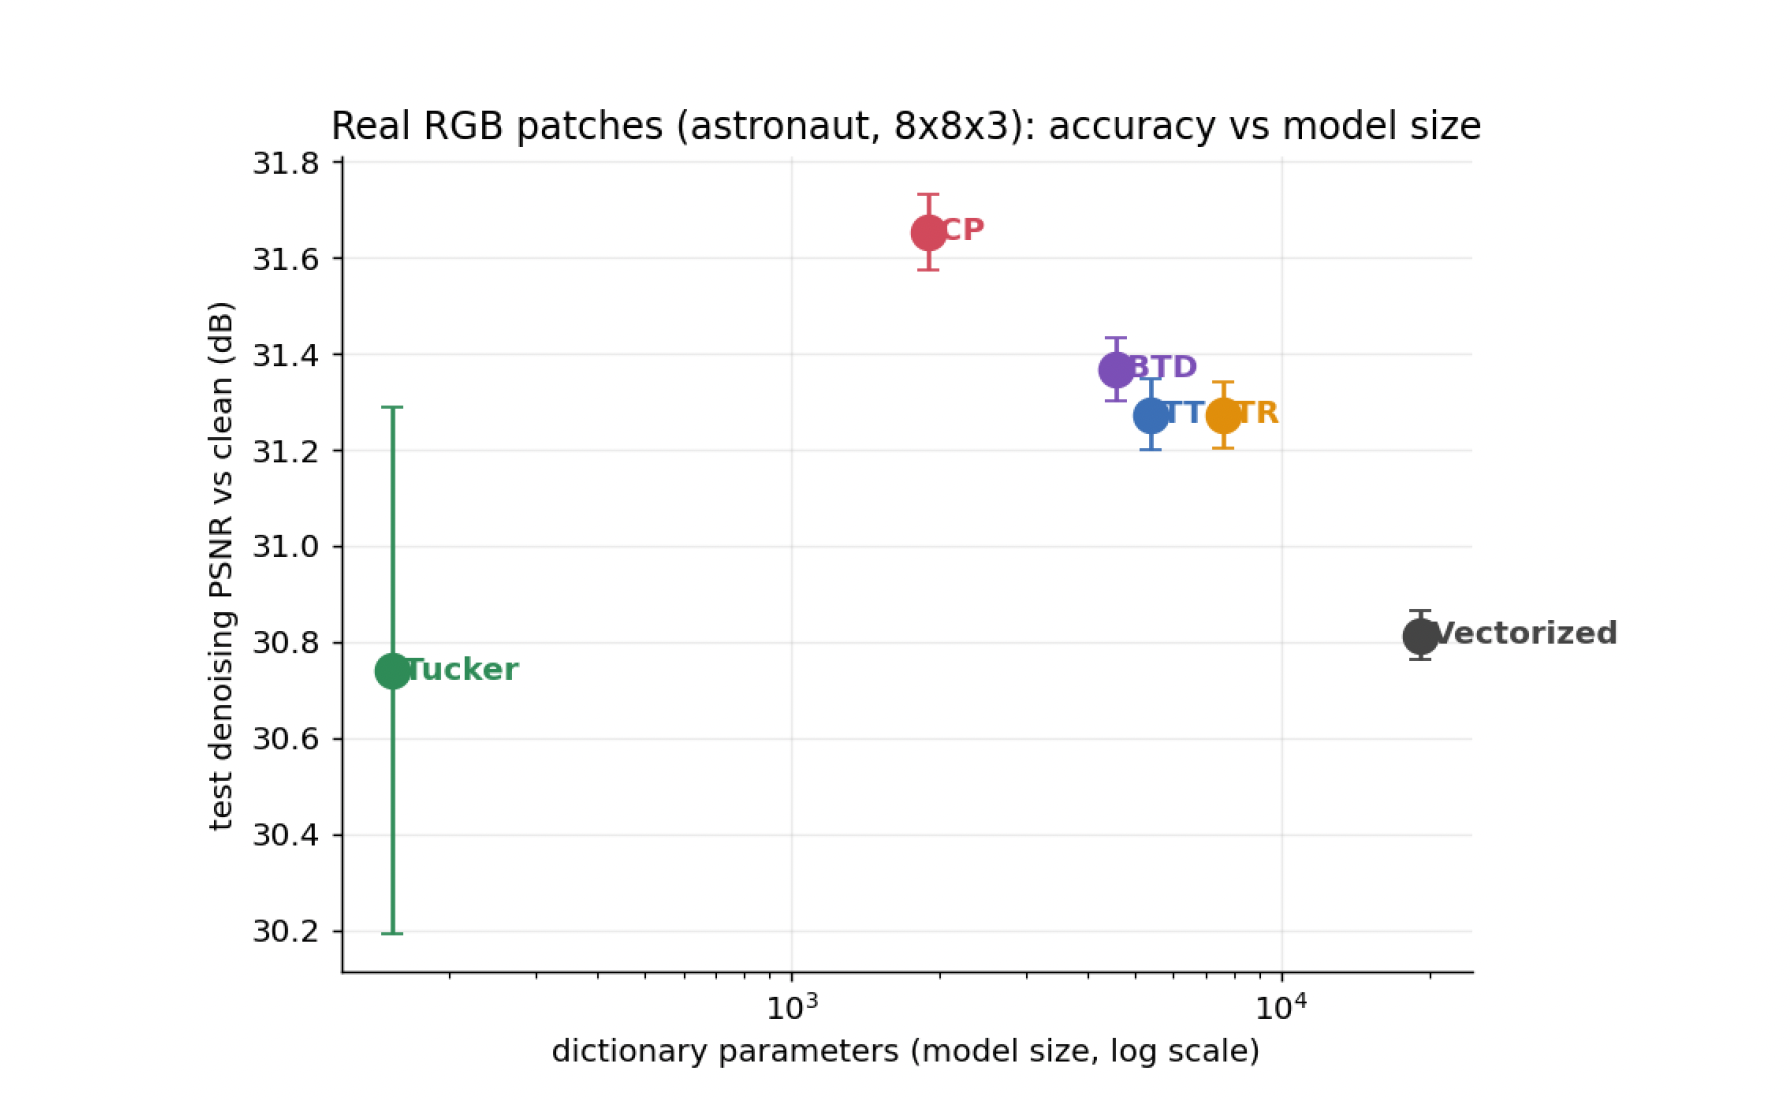
\includegraphics[width=0.78\textwidth]{figures/fig09_frontier_rgb.png}

\credit{Figure 9 --- structured dictionaries move above the vectorized baseline.}
\end{column}
\end{columns}
\takeaway{\textbf{31.65\dB{} vs 30.81\dB} --- the vectorized dictionary spends its
extra capacity fitting noise; the structured methods \emph{cannot}, so their
constraint accidentally acts as a regularizer.}
\end{frame}

\begin{frame}{CP instability: accuracy can hide a degenerate factorization}
\centering
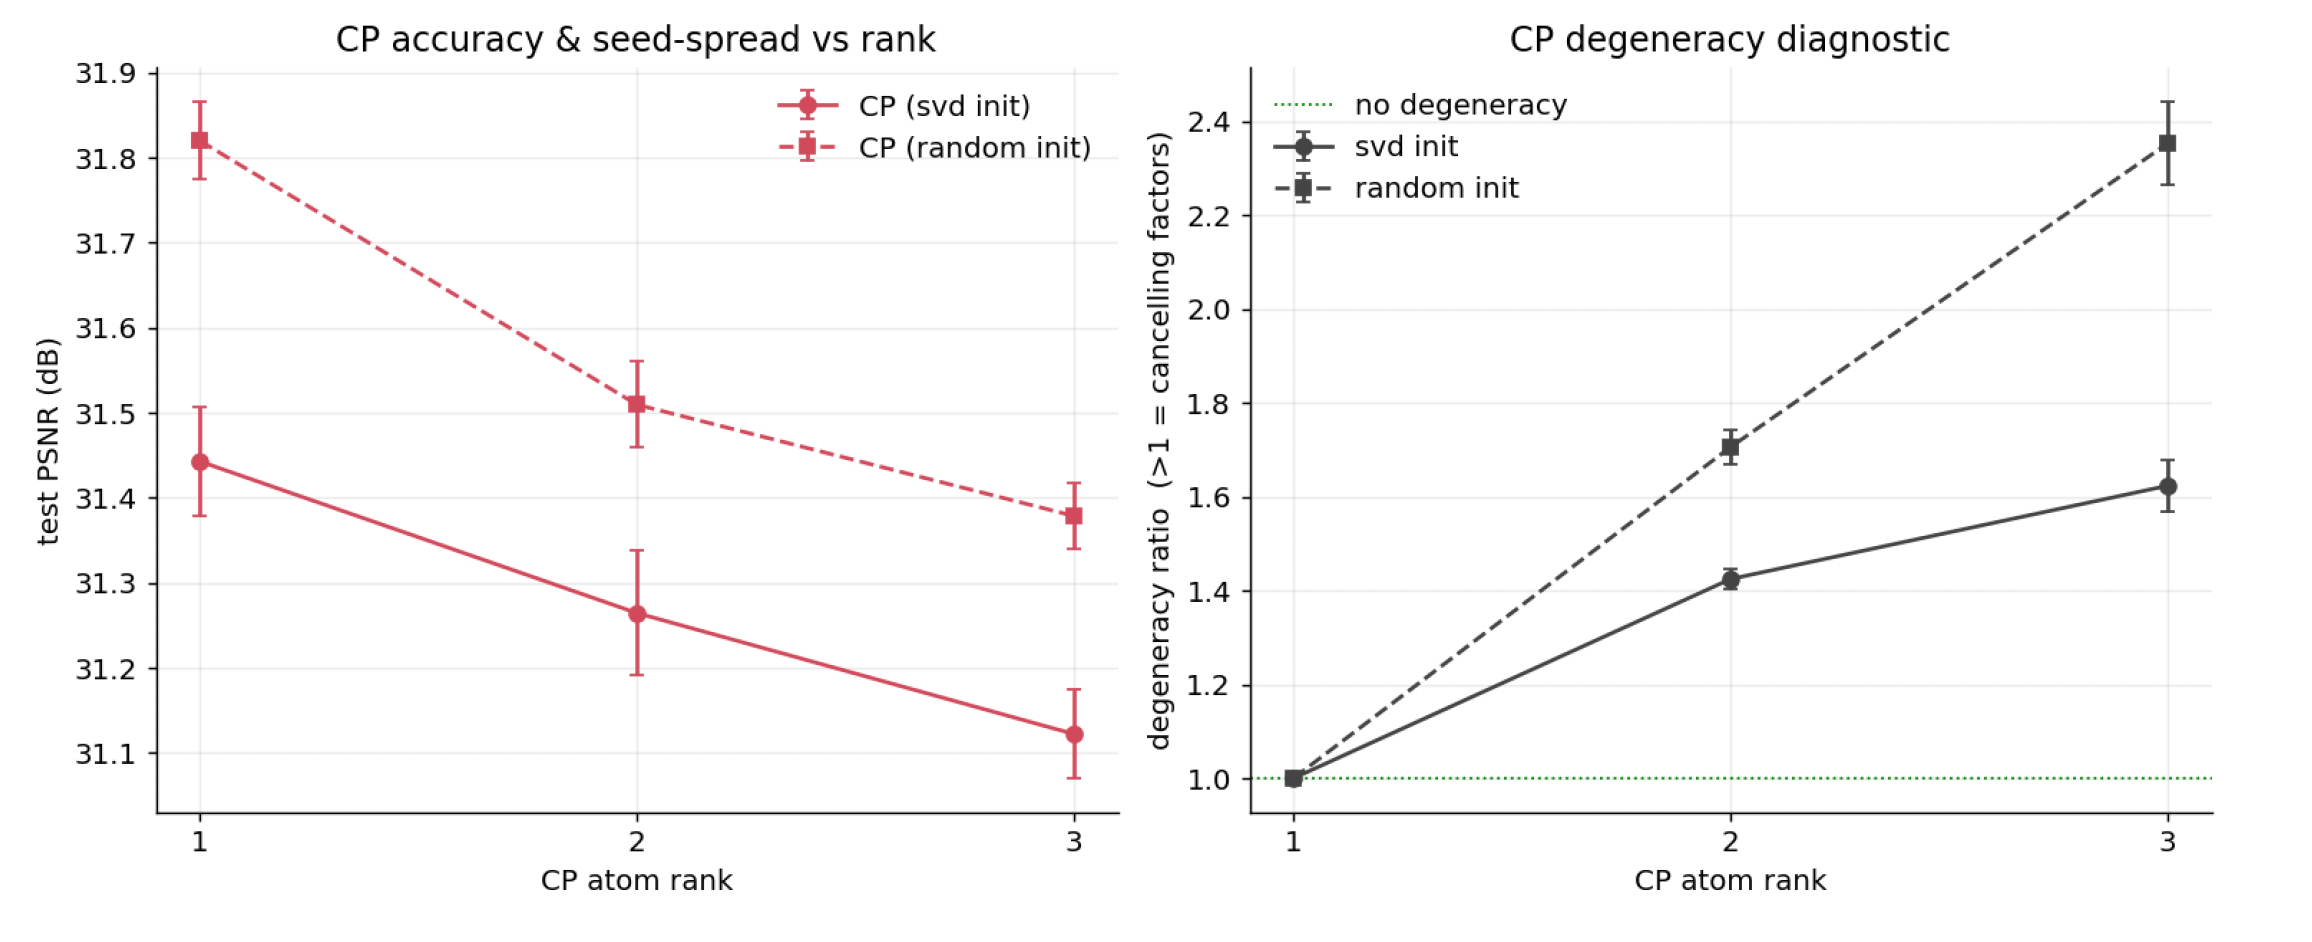
\includegraphics[width=0.80\textwidth]{figures/fig10_cp_instability.png}

\credit{Figure 10 --- left: accuracy and seed-spread versus rank for SVD vs
random initialization. Right: the degeneracy diagnostic climbs with rank.}

\smallskip
\scriptsize
The degeneracy ratio is the sum of component magnitudes over the norm of their
sum. Rank-one atoms are always non-degenerate ($=1.0$); the ratio grows with rank,
with random init producing markedly more degenerate, partially cancelling
components than an SVD warm start (2.35 vs 1.62 at rank 3). Reconstruction can
look fine while the factorization is internally degenerate --- a warning if the
factors are used downstream.
\end{frame}

\begin{frame}{BTD interpolates CP and Tucker}
\begin{columns}[T,onlytextwidth]
\begin{column}{0.50\textwidth}
\centering
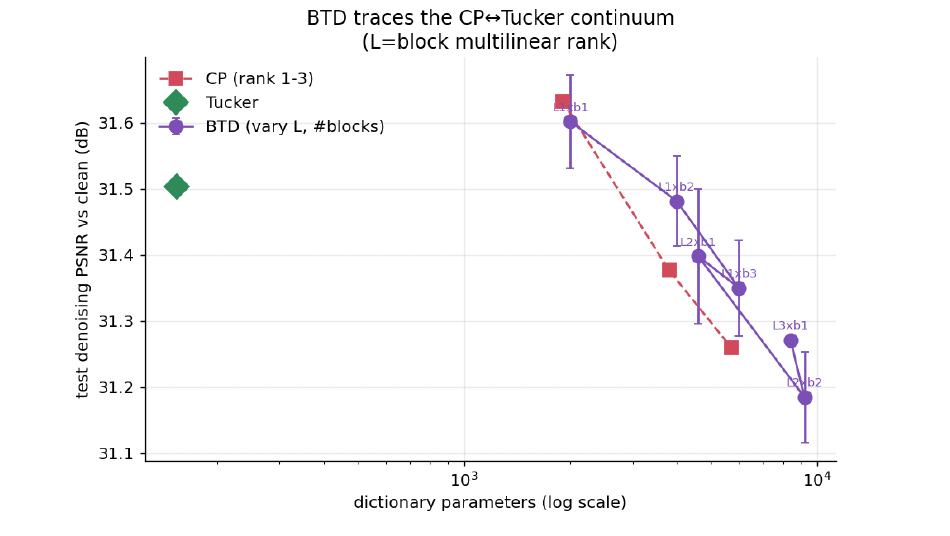
\includegraphics[width=0.92\textwidth]{figures/fig11_btd_continuum.png}

\credit{Figure 11 --- BTD traces the CP $\leftrightarrow$ Tucker continuum as
block rank $L$ and block count vary.}
\end{column}
\begin{column}{0.46\textwidth}
\small
The $L{=}1$, one-block configuration lands exactly on CP rank-one, confirming the
endpoint identity, and the family traces the continuum toward Tucker. In this
noisy regime the most constrained point is best --- extra capacity fits noise.
\medskip

Tucker stays almost stationary because its parameter count grows far more slowly
than its dictionary size: unlike CP and BTD, which add parameters per atom,
Tucker stores only three shared mode dictionaries. Parameters grow roughly
linearly with mode dimension while the atom count grows multiplicatively.
\end{column}
\end{columns}
\end{frame}

%=======================================================================
\section{Refinement of the Tucker Optimizer}
%=======================================================================

\begin{frame}{An optimizer bug, not a structural verdict}
\small
The original Tucker-DL failed on an \textbf{objective mismatch}: it learned its
three mode dictionaries in isolation,
\[ Y_{(1)} \approx U_1 X_1, \qquad Y_{(2)} \approx U_2 X_2, \qquad Y_{(3)} \approx U_3 X_3, \]
but a Tucker dictionary is never seen alone --- only as
$D = U_3 \kron U_2 \kron U_1$. The fix keeps OMP against the Kronecker dictionary
and updates by separable ALS: solve $U_1$ with $(U_2,U_3)$ fixed, then $U_2$,
then $U_3$, each an \emph{exact closed-form least-squares} block.

\medskip
\begin{columns}[T,onlytextwidth]
\begin{column}{0.48\textwidth}
\begin{exampleblock}{RGB patches}
\centering $30.66\dB \;\longrightarrow\; 32.16 \pm 0.09\dB$

\credit{at an identical 153-parameter budget}
\end{exampleblock}
\end{column}
\begin{column}{0.48\textwidth}
\begin{exampleblock}{Synthetic data}
\centering $27.01\dB \;\longrightarrow\; 29.45 \pm 0.69\dB$

\credit{a gain of approximately $+1.5\dB$}
\end{exampleblock}
\end{column}
\end{columns}
\takeaway{A fairness correction to one optimizer moved Tucker from last place to
a Pareto-dominant winner at identical size.}
\end{frame}

\begin{frame}{Efficiency ranking with the corrected Tucker: RGB}
\begin{columns}[T,onlytextwidth]
\begin{column}{0.47\textwidth}
\centering\scriptsize
\begin{tabular}{@{}lrrrccr@{}}
\toprule
\textbf{Model} & \textbf{PSNR} & \textbf{Params} & \textbf{$E$} & \textbf{Par.} & \textbf{Tier} & \textbf{Bal.}\\
\midrule
Tucker     & 32.16 & 153      & 14.72 & yes & S & 0.892 \\
CP         & 31.71 & 1{,}900  & 9.67  & no  & C & 0.429 \\
TT         & 31.28 & 5{,}400  & 8.38  & no  & C & 0.389 \\
BTD        & 31.38 & 4{,}600  & 8.57  & no  & C & 0.385 \\
TR         & 31.31 & 7{,}600  & 8.07  & no  & C & 0.306 \\
Vectorized & 30.80 & 19{,}200 & 7.19  & no  & D & 0.230 \\
\bottomrule
\end{tabular}

\medskip
\credit{Table 5 --- corrected Tucker, 5 seeds,
$E = \mathrm{PSNR}/\log_{10}(\mathrm{params})$. \textbf{Caveat:} Tucker's
$9\times9\times3$ grid yields 243 implicit atoms for 153 explicit parameters,
where other methods get $\approx$100 atoms at the same count --- part of its edge
is extra atoms at the same sparsity level.}
\end{column}
\begin{column}{0.49\textwidth}
\centering
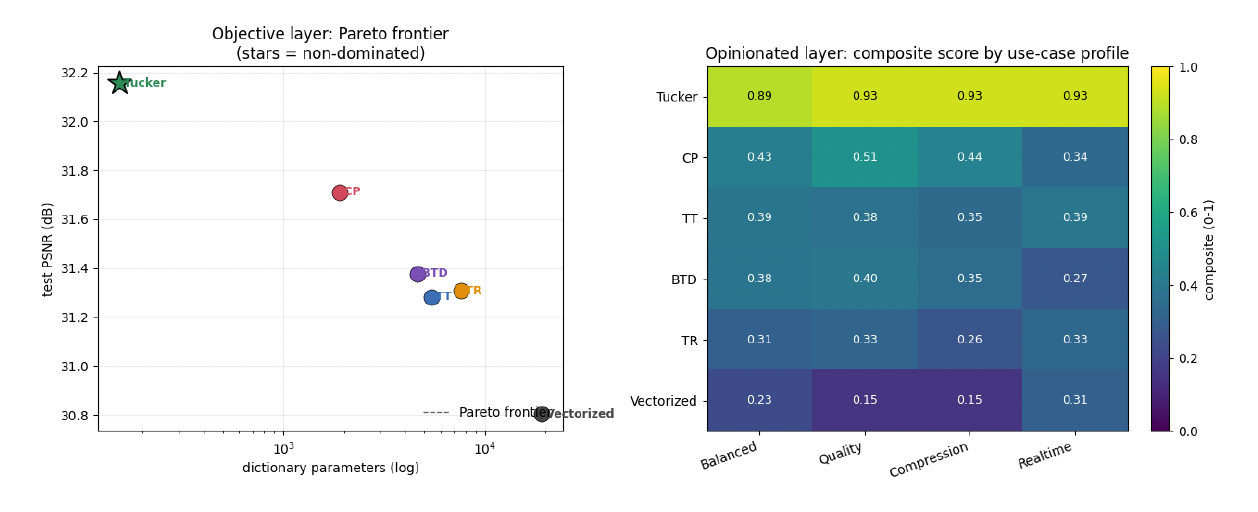
\includegraphics[width=\textwidth]{figures/fig12_ranking_rgb.png}

\credit{Figure 12 --- left: objective Pareto layer (stars are non-dominated);
only Tucker is on the frontier. Right: profile-weighted composite scores.}
\end{column}
\end{columns}
\end{frame}

\begin{frame}{Efficiency ranking with the corrected Tucker: synthetic}
\begin{columns}[T,onlytextwidth]
\begin{column}{0.43\textwidth}
\centering\scriptsize
\begin{tabular}{@{}lrrrcc@{}}
\toprule
\textbf{Model} & \textbf{PSNR} & \textbf{Params} & \textbf{$E$} & \textbf{Tier} & \textbf{Bal.}\\
\midrule
Vectorized & 41.25 & 25{,}920 & 9.35  & A & 0.700 \\
TR         & 36.98 & 8{,}640  & 9.39  & C & 0.413 \\
TT         & 36.46 & 5{,}760  & 9.70  & B & 0.482 \\
CP         & 32.65 & 2{,}160  & 9.79  & C & 0.417 \\
Tucker     & 29.45 & 126      & 14.02 & C & 0.416 \\
\bottomrule
\end{tabular}

\medskip
\credit{Table 6 --- in-harness Tucker, 5 seeds. Every method is Pareto-optimal:
the frontier is monotone, so the objective layer prunes nothing.}
\end{column}
\begin{column}{0.53\textwidth}
\centering
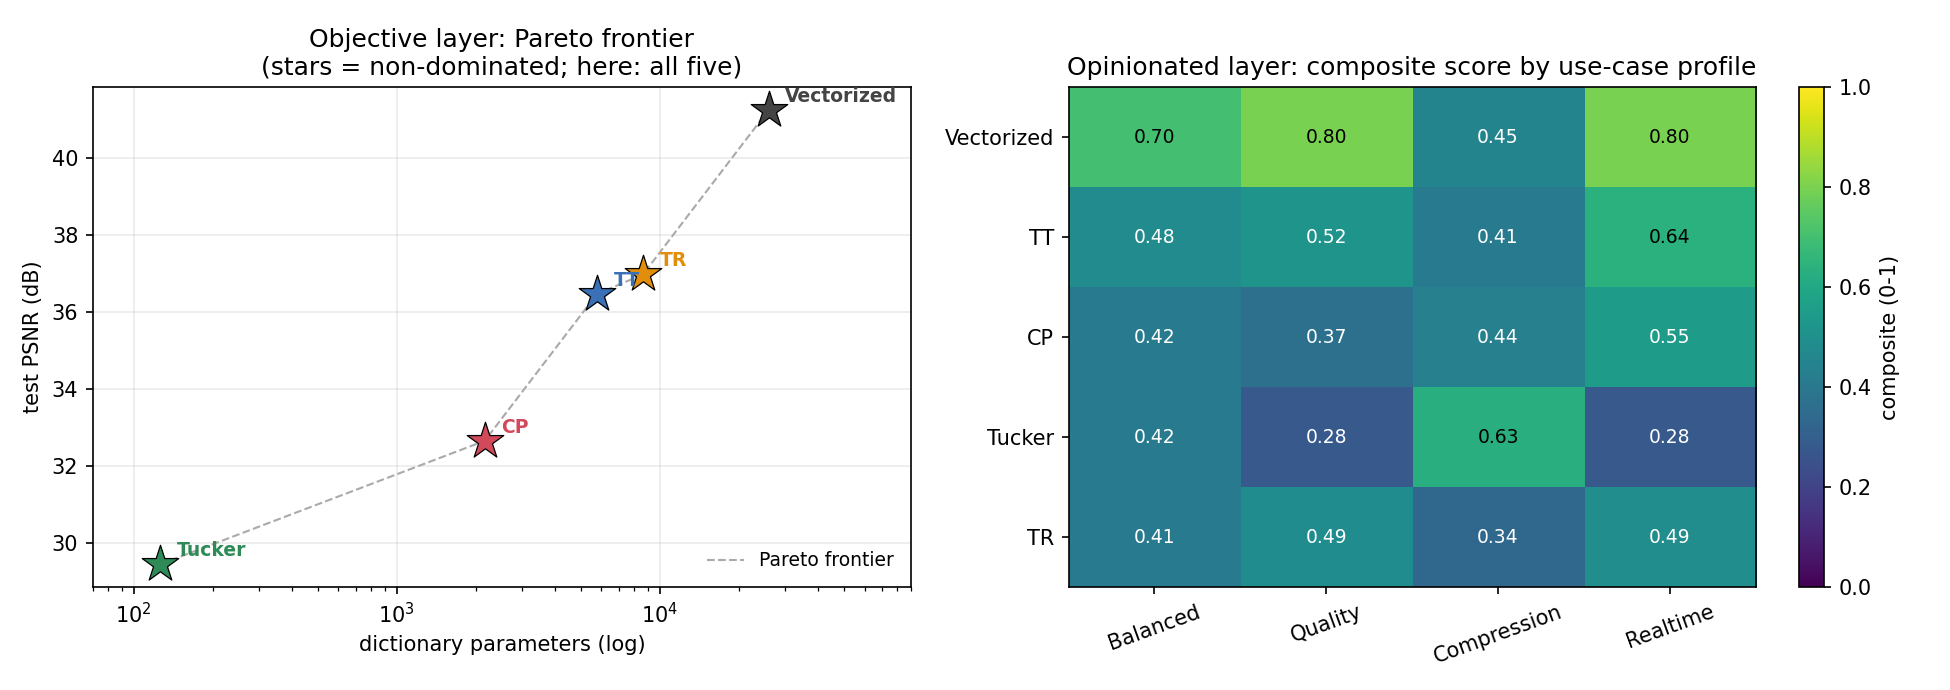
\includegraphics[width=\textwidth]{figures/fig13_ranking_synthetic.png}

\credit{Figure 13 --- with a monotone frontier, all the discriminating work falls
to the opinionated layers.}
\end{column}
\end{columns}
\end{frame}

%=======================================================================
\section{Results 3: Matched-Budget Hyperspectral}
%=======================================================================

\begin{frame}{Matched parameter budget removes the hand-picked ranks}
\begin{columns}[T,onlytextwidth]
\begin{column}{0.52\textwidth}
\centering
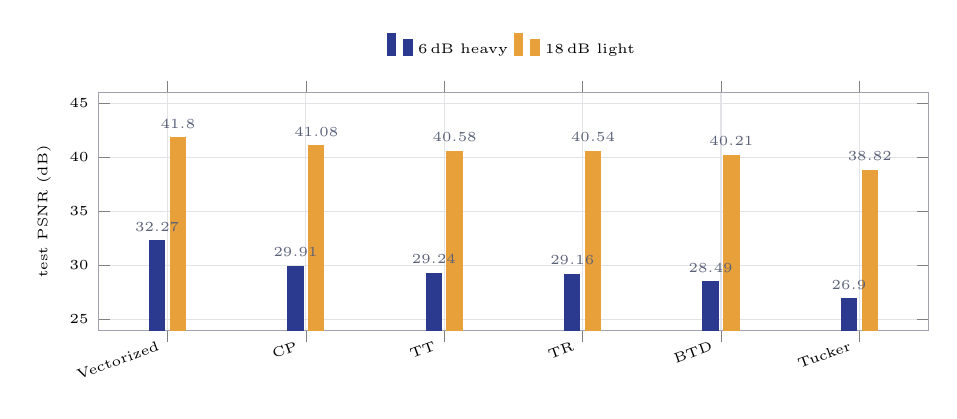
\begin{tikzpicture}
\begin{axis}[
  width=\textwidth, height=4.6cm,
  ybar, bar width=5.5pt,
  ymin=24, ymax=46,
  symbolic x coords={Vectorized,CP,TT,TR,BTD,Tucker},
  xtick=data,
  x tick label style={font=\tiny, rotate=20, anchor=east},
  y tick label style={font=\tiny},
  ylabel={test PSNR (dB)}, ylabel style={font=\tiny},
  legend style={font=\tiny, at={(0.5,1.10)}, anchor=south, legend columns=2, draw=none},
  grid=major, grid style={draw=ink!12},
  axis line style={draw=ink!40},
  nodes near coords, every node near coord/.append style={font=\tiny, color=muted},
]
\addplot[fill=indigo, draw=indigo] coordinates
  {(Vectorized,32.27) (CP,29.91) (TT,29.24) (TR,29.16) (BTD,28.49) (Tucker,26.90)};
\addplot[fill=amber, draw=amber] coordinates
  {(Vectorized,41.80) (CP,41.08) (TT,40.58) (TR,40.54) (BTD,40.21) (Tucker,38.82)};
\legend{6\dB{} heavy, 18\dB{} light}
\end{axis}
\end{tikzpicture}

\credit{Table 7 --- HSI cube $6\times6\times16$ at the
$\approx$5{,}000-parameter slice. Tucker operates at 304 parameters: it cannot
reach the budget without exceeding a reasonable atom cap.}
\end{column}
\begin{column}{0.44\textwidth}
\begin{block}{A fat mode is not a high order}
\scriptsize Giving Tensor-Train a large third mode did \emph{not} hand it the
win. TT's advantage is high tensor \emph{order}, not one wide mode.
\end{block}
\begin{block}{The ranking does not flip with noise}
\scriptsize Between heavy (6\dB) and light (18\dB) noise only the absolute PSNR
shifts; the ordering is stable.
\end{block}
\begin{block}{Less is more on a low-rank cube}
\scriptsize Accuracy falls as the budget grows. The baseline leads at 5{,}000
parameters partly because its atoms cost 576 each.
\end{block}
\end{column}
\end{columns}
\end{frame}

\begin{frame}{Why the matched-budget study is restricted to HSI}
\small
\begin{itemize}\setlength\itemsep{0.8em}
  \item \textbf{Isolating the wide mode.} The experiment tests whether
        Tensor-Train benefits from a single wide mode or from higher-order
        structure. The $6\times6\times16$ HSI tensor is the only dataset in the
        benchmark that provides a wider mode in isolation.
  \item \textbf{Selection bias needs a validation split.} Choosing ranks on
        training reconstruction error would unfairly favour larger, less
        regularized models. HSI is split into training, validation and test: each
        configuration trains on the training set, the rank is chosen on
        validation, and the selected model is evaluated \emph{once} on test.
  \item \textbf{Scope.} These considerations justify restricting the analysis to
        HSI, but the conclusions apply to this experimental setting rather than
        universally.
\end{itemize}
\end{frame}

\begin{frame}{Rate--distortion sweep across noise levels}
\centering
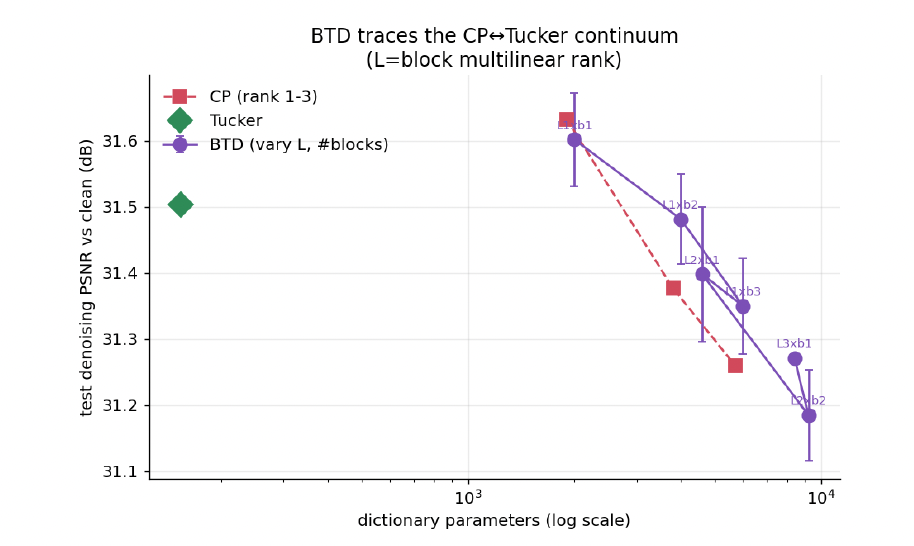
\includegraphics[width=0.52\textwidth]{figures/fig14_matched_budget.png}

\credit{Figure 14 as printed in the manuscript.}

\smallskip
\scriptsize
\textcolor{rust}{\textbf{Note:}} the embedded image duplicates Figure 11 (the BTD
continuum). The caption describes the matched-budget rate--distortion curve at
6\dB{} and 18\dB, whose numbers appear on the previous slide --- worth
regenerating before submission.
\end{frame}

%=======================================================================
\section{Discussion}
%=======================================================================

\begin{frame}{Three themes}
\begin{block}{(i) Regime dependence}
\small There is no absolute best decomposition. The baseline wins on rich clean
synthetic data; structured dictionaries win on noisy real patches where their
constraint regularizes; at matched budget on a low-rank cube, few full atoms or a
tiny Tucker are most efficient. Which to use is a function of signal order, noise
and intrinsic rank --- not a fixed ranking.
\end{block}
\begin{block}{(ii) Confounds can dominate structure}
\small The Tucker rebuild moved it from last to first at identical size purely by
fixing the optimizer, and the matched-budget study revised the earlier
``structured wins'' story by revealing that some of that advantage was really the
freedom to buy many cheap atoms.
\end{block}
\begin{block}{(iii) Matched-parameter is not matched-atom}
\small At equal storage the baseline is forced into few heavily regularized atoms
while structured methods spend the same budget on many. Which budget is ``fair''
depends on whether you care about storage or per-atom quality.
\end{block}
\end{frame}

\begin{frame}{Limitations}
\begin{columns}[T,onlytextwidth]
\begin{column}{0.48\textwidth}
\begin{block}{Implementations, not canonical algorithms}
\scriptsize CP/TT/TR/BTD here are projection variants inside a shared K-SVD loop
--- not jointly optimized factors, PALM-based TT-DL or SeDiL. The numbers rank
these implementations, not those methods definitively.
\end{block}
\begin{block}{Modest data, seed-only error bars}
\scriptsize Hundreds of patches, single images, a few noise levels; the bars
capture seed variance alone, and the HSI cube is synthetic.
\end{block}
\end{column}
\begin{column}{0.48\textwidth}
\begin{block}{The budget study caps atom counts}
\scriptsize Capping for tractability bounds Tucker artificially --- it is why
Tucker sits at the far left of the rate--distortion curve rather than on it.
\end{block}
\begin{block}{The speed axis understates tensor methods}
\scriptsize The harness materializes the full effective dictionary and runs
identical OMP for fairness, discarding the fast structured transforms that are a
genuine advantage of Kronecker and TT dictionaries.
\end{block}
\end{column}
\end{columns}
\takeaway{A fuller treatment would report several implementations per structure
and show the spread --- natural next steps rather than flaws to hide.}
\end{frame}

\begin{frame}[standout]
One harness, six dictionaries,\\
and a ranking that can be re-derived anywhere
\end{frame}

\begin{frame}{Conclusion}
\begin{columns}[T,onlytextwidth]
\begin{column}{0.31\textwidth}
\begin{block}{Connected}
\small Five tensor-structured dictionaries and an unstructured baseline differing
only in how each atom is parameterized --- linked to DL through the Khatri--Rao
and Kronecker forms.
\end{block}
\end{column}
\begin{column}{0.31\textwidth}
\begin{block}{Measured}
\small Across synthetic, real and hyperspectral data the best decomposition is
regime-dependent, and implementation confounds can outweigh structural
differences.
\end{block}
\end{column}
\begin{column}{0.31\textwidth}
\begin{block}{Extensible}
\small A matched parameter budget both tightens and, in places, reverses naive
conclusions. A new decomposition is one projector and one parameter rule away.
\end{block}
\end{column}
\end{columns}
\vfill
\centering\small Sahaj Chhetri \quad$\cdot$\quad August 17, 2026
\quad$\cdot$\quad Primitives via TensorLy
\end{frame}

\begin{frame}[allowframebreaks]{References}
\footnotesize
\begin{thebibliography}{10}
\bibitem{ksvd} M.~Aharon, M.~Elad, and A.~Bruckstein. K-SVD: An algorithm for
  designing overcomplete dictionaries for sparse representation.
  \emph{IEEE Trans. Signal Processing}, 2006.
\bibitem{omp} Y.~C. Pati, R.~Rezaiifar, and P.~S. Krishnaprasad. Orthogonal
  matching pursuit. \emph{Asilomar Conf. on Signals, Systems and Computers}, 1993.
\bibitem{kolda} T.~G. Kolda and B.~W. Bader. Tensor decompositions and
  applications. \emph{SIAM Review}, 2009.
\bibitem{tucker} L.~R. Tucker. Some mathematical notes on three-mode factor
  analysis. \emph{Psychometrika}, 1966.
\bibitem{tt} I.~V. Oseledets. Tensor-train decomposition.
  \emph{SIAM J. Scientific Computing}, 2011.
\bibitem{tr} Q.~Zhao, G.~Zhou, S.~Xie, L.~Zhang, and A.~Cichocki. Tensor ring
  decomposition. \emph{arXiv:1606.05535}, 2016.
\bibitem{btd} L.~De~Lathauwer. Decompositions of a higher-order tensor in block
  terms --- Part II. \emph{SIAM J. Matrix Analysis and Applications}, 2008.
\bibitem{sep} S.~Hawe, M.~Seibert, and M.~Kleinsteuber. Separable dictionary
  learning. \emph{CVPR}, 2013.
\bibitem{kron} C.~F. Caiafa and A.~Cichocki. Computing sparse representations of
  multidimensional signals using Kronecker bases. \emph{Neural Computation}, 2013.
\bibitem{tensorly} J.~Kossaifi, Y.~Panagakis, A.~Anandkumar, and M.~Pantic.
  TensorLy: Tensor learning in Python. \emph{JMLR}, 2019.
\end{thebibliography}
\end{frame}

\end{document}
